\nonstopmode
\documentclass[10pt, a4paper]{article}
\parindent=20pt
\parskip=8pt
\usepackage[width=15.5cm, left=3cm, top=2.5cm, height= 24.5cm]{geometry}
\usepackage[spanish]{babel}
\usepackage[utf8]{inputenc}
\usepackage{fancyhdr}
\usepackage{latexsym}
\usepackage{caratula}
\usepackage{epsfig}
%\usepackage{algorithmicx}
\usepackage{lastpage}
\usepackage{amsfonts}
\usepackage{listings}
\usepackage{algorithm}
\usepackage{algpseudocode}
\usepackage{pdfpages}
\usepackage{amsmath}
\usepackage{verbatim}
\usepackage{graphicx}
\usepackage{float}
\graphicspath{{imgs/}}

% Acomodo fancyhdr.
\pagestyle{fancy}
\thispagestyle{fancy}
\addtolength{\headheight}{1pt}
\lhead{Teor\'ia de las Comunicaciones}
\rhead{TP1}
\cfoot{\thepage /\pageref{LastPage}}
\renewcommand{\footrulewidth}{0.4pt}
\renewcommand{\thesubsubsection}{\thesubsection.\alph{subsubsection}}


\author{Teor\'ia de las Comunicaciones, DC, UBA.}
\date{}
\title{}

\begin{document}
	
\thispagestyle{empty}
\materia{Teor\'ia de las Comunicaciones}
%\submateria{Trabajo Pr\'actico Nº1}
\titulo{Trabajo Práctico Nº2}
\integrante{Rivero, Maximiliano}{366/07}{maxirivero088@gmail.com}
\integrante{Izcovich, Sabrina}{550/11}{sizcovich@gmail.com}
\integrante{Rogani, Marcos}{520/05}{marcos.rogani@gmail.com}

\maketitle

\tableofcontents
\newpage

\section{Introducción}

En el siguiente trabajo práctico, experimentamos $traceroute$ con herramientas y técnicas frecuentes a nivel de red. Para ello, implementamos en primer lugar una $tool$ que mitiera realizar un $traceroute$ mediante sucesivos paquetes con TTLs incrementales, calculando los RTTs entre cada salto para los que se reciba una respuesta ICMP de tipo $time exceeded$. 

Luego, adaptamos la $tool$ realizada para que, una vez terminada la búsqueda, calculara el valor standard o valor Z del RTT (ZRTT) de cada salto $i$ con respecto a la ruta global de la siguiente manera: 
$$ZRTT_i = \frac{RTT_i - \overline{RTT}}{SRTT}$$
siendo $\overline{RTT}$ y $SRTT$ el promedio y el desvío standard de los RTTs de la ruta, respectivamente. Por otra parte, los $RTT_i$ corresponden al tiempo de ida y vuelta dentre el hop $i$ y el hop $i-1$, siendo éstos consecutivos.

Por último, utilizamos la $tool$ para estudiar y analizar rutas a universidades en diferentes lugares del mundo.

Para un análisis adecuado, realizamos gráficos de distribuciones de RTTs estudiando qué saltos son estadísticamente significativos con respecto a la ruta analizada. A partir de esta herramienta, detectamos saltos correspondientes a enlaces submarinos, entre otros. 

\section{Introducción Teórica}
\begin{itemize}
\item \textbf{ICMP(Internet Control Message Protocol):} Protocolo de control que forma parte del núcleo de la arquitectura TCP/IP. El mismo se encarga de proveer mensajes de error y de control. Éstos son:
\begin{itemize}
\item Errores en los datagramas IP.
\item Necesidad de comunicar información de diagnóstico.
\item Necesidad de comunicar información de ruteo.
\end{itemize}
Los paquetes constan de una sección de datos y un header con la siguiente estructura:

\begin{figure}[H] %[h] Aqui [b] para button [t] para top
\begin{center}
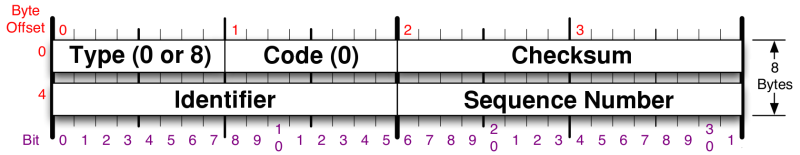
\includegraphics[width=400pt]{../imgs/icmp.png}
\caption{Header de ICMP.}
\end{center}
\end{figure}

\item \textbf{Mensajes de control de ICMP}:
Los mensajes de control que analizaremos a lo largo del trabajo son los siguientes:
\begin{itemize}
\item \textbf{Echo Reply (tipo 0)}: Consiste en un mensaje generado como respuesta a un mensaje Echo Request (petición de Eco).
\item \textbf{Echo Request (tipo 8)}: Consiste en un mensaje de control que se envía a un host con la expectativa de recibir de él un Echo Reply (Respuesta eco).
\item \textbf{Time Exceeded (tipo 11)}: Consiste en un mensaje que se utiliza para indicar que el tiempo de vida de un paquete llegó a su fin.
\end{itemize}

\item \textbf{Round-Trip Time}: Corresponde al retardo del tránsito de paquetes a través de la red IP desde que es enviado hasta volver al emisor, pasando por el destino.

\item \textbf{Traceroute}: Consiste en una herramienta de diagnóstico que muestra la ruta y mide el RTT.
\end{itemize}

\section{Desarrollo}
Para la implementación del traceroute, seguimos el siguiente algoritmo:

\begin{algorithm}
\caption{Algoritmo de Traceroute}
\begin{algorithmic}
\Procedure{traceroute}{$IP_{dst}$}

\State $h\gets IP_{dst}$
\State $ttl\gets 1$
\State $anotadas \gets \{\}$
\Repeat
	\State $h.TTL \gets ttl$
	\State $enviar(h, EchoRequest, TimeOut)$
	\If {$obtener(TimeExceeded)\ \&\&\ \neg obtener(TimeOut)$}
    	\State $anotadas.push(IP_{rcv})$
    \Else
    	\State $anotadas.push(^*)$
    \EndIf
    \State $ttl\gets ttl+1$
\Until{$IP_{dst} = IP_{rcv}$}
\EndProcedure
\end{algorithmic}
\end{algorithm}

donde $h$ representa el host destino e $IP_{rcv}$ representa la IP del hop del que proviene el paquete recibido. Por otro lado, $ttl$ representa el \textit{time to live} del paquete y $TTL$ el campo correspondiente en el header del mismo.

Para la segunda parte del análisis, modificamos la implementación con el fin de que, una vez terminada la búsqueda, calculara el valor standard o valor Z del RTT (ZRTT) de cada salto $i$ con respecto a la ruta global. El cambio dio como resultado el siguiente algoritmo:

\begin{algorithm}
\caption{Algoritmo de Traceroute con ZRTT}
\begin{algorithmic}
\Procedure{traceroute}{$IP_{dst}$}

\State $h\gets IP_{dst}$
\State $ttl\gets 1$
\State $anotadas \gets \{\}$
\State $RTTs \gets \{\}$
\Repeat
	\State $h.TTL \gets ttl$
	\State $enviar(h, EchoRequest, TimeOut)$
	\State $clock.reset()$
	\If {$obtener(TimeExceeded)\ \&\&\ \neg obtener(TimeOut)$}
    	\State $anotadas.push(IP_{rcv})$
    \Else
    	\State $anotadas.push(^*)$
    \EndIf
    \State $RTTs_i \gets clock.now()$
    \State $ttl\gets ttl+1$
    \State $ZRTT_i \gets \frac{RTTs_i - promedio(RTTs)}{standDesv(RTTs)}$
\Until{$IP_{dst} = IP_{rcv}$}
\EndProcedure
\end{algorithmic}
\end{algorithm}

Las implementaciones se realizaron en python.

\section{Resultados}


\newpage
\section{Discusión}

\section{Conclusiones}


\section{Referencias}
\begin{itemize}
\item PETERSON, DAVIE ; Computer Networks, 5th edition, Wiley


\end{itemize}
\end{document}
